\subsection{Kolonnefamiliedatabase}
Cassandra er verktøyet vi skulle bruke for å opprette Kolonnefamiliedatabaser. Fra tidligere hadde vi allerede designet aggregeringene og laget de via spark-shell i Scala, så prossessen var heldigvis rett fram. For alle aggregeringene, inkluderende rådataen, måtte man opprette en ny table/kolonnefamilie i Cassandra med samsvarende kolonnenavn og datatype.

\subsubsection{Opprette keyspace}
Det første må gjøre er å opprette et "keyspace" i Cassandra. Dette tilsvarer en database i MySQL. Her opprettes keyspacet "university" hvor alle kommende tables havner i. Det er viktig å merke seg \lstinline{WITH replication}, siden den bestemmer hvordan datakopier spres utover en klynge. For denne løsning brukes \textit{SimpleStrategy} med \textit{replication factor} av 1. 

\txt{code/createNamespace.txt}

Replikasjonsstrategien bestemmer hvordan datakopiene distribueres rundt om i \textit{Cassandra ringen}, der en ring representerer en klynge av noder, også kalt et datasenter. Som en tommelfingelregel brukes SimpleStrategy når man bare har et datasenter, ellers brukes \textit{NetworkTopologyStrategy}. Begge strategiene populerer datasettene node for node med klokken, forskjellen er at SimpleStrategy kun populerer et datasett, mens NetworkTopologyStrategy populererer flere.

\begin{figure}[H]
  \centering
  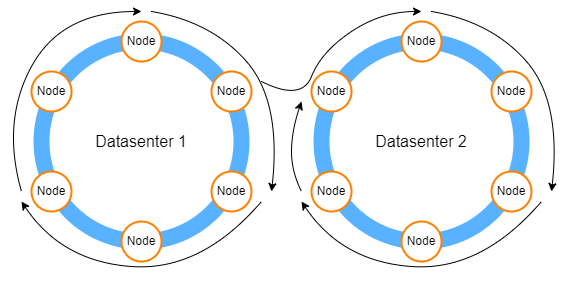
\includegraphics[scale=0.5]{images/replicationstrategy.drawio.png}
  \caption{Figuren viser hvordan de to replikasjonsstrategiene distribuerer datakopier utover klyngene. SimpleStrategy vil kun distribuere til datasenter 1, mens NetworkTopologyStrategy vil starte i datasenter 1 og jobbe seg utover datasenter 2.}
\end{figure}

Videre bestemmer replikasjonsfaktoren hvor mange datakopier som skal spres utover klyngen, for eksempel i en klynge med seks noder og replikasjonsfaktor på tre, vil halvparten av nodene være tilgitt en datakopi. På denne måten forsørger man at data er utilgjengelig dersom en node skulle feile. Legg merke til at det ikke er lov til å ha en replikasjonsfaktor større enn antall noder i en klynge. 

I Cassandra tar man også hensyn til noe kalt for \textit{Cassandra consistensy level}, som er minimum antall noder som må annerkjenne lese- og skrive-spørringer før det kan kalles en gyldig operasjon. Dette er en verdi som kan settes selv. Som regel brukes Cassandra verdien \textit{Local Quorum}, som defineres slik: \lstinline{LOCAL_QUORUM = (replication_factor/2) + 1}, denne rundes ned til nærmeste heltall.

\subsubsection{Opprette kolonnefamilier i Cassandra}
\txt{code/createTable.txt}

\subsubsection{Laste opp rådata}
\code{Scala}{code/populateCassandraRaw.scala}

%\code{Scala}{code/populateCassandraFemaleRatio.scala}
%\code{Scala}{code/populateCassandraMaleRatio.scala}
%\code{Scala}{code/populateCassandraAverageScorePerYear.scala}